%%%%%%%%%%%%%%%%%%%%%%%%%%%%%%%%%%%%%%%%%
% Beamer Presentation
% LaTeX Template
% Version 1.0 (10/11/12)
%
% This template has been downloaded from:
% http://www.LaTeXTemplates.com
%
% License:
% CC BY-NC-SA 3.0 (http://creativecommons.org/licenses/by-nc-sa/3.0/)
%
%%%%%%%%%%%%%%%%%%%%%%%%%%%%%%%%%%%%%%%%%

%----------------------------------------------------------------------------------------
%	PACKAGES AND THEMES
%----------------------------------------------------------------------------------------

\documentclass{beamer}
\usefonttheme[onlymath]{serif}

\usepackage{color}
\usepackage{lmodern}
\usepackage{graphicx}
\usepackage{tikz}

\mode<presentation> {

% The Beamer class comes with a number of default slide themes
% which change the colors and layouts of slides. Below this is a list
% of all the themes, uncomment each in turn to see what they look like.

%\usetheme{default}
%\usetheme{AnnArbor}
%\usetheme{Antibes}
%\usetheme{Bergen}
%\usetheme{Berkeley}
%\usetheme{Berlin}
\usetheme{Boadilla}
%\usetheme{CambridgeUS}
%\usetheme{Copenhagen}
%\usetheme{Darmstadt}
%\usetheme{Dresden}
%\usetheme{Frankfurt}
%\usetheme{Goettingen}
%\usetheme{Hannover}
%\usetheme{Ilmenau}
%\usetheme{JuanLesPins}
%\usetheme{Luebeck}
% \usetheme{Madrid}
%\usetheme{Malmoe}
%\usetheme{Marburg}
%\usetheme{Montpellier}
%\usetheme{PaloAlto}
%\usetheme{Pittsburgh}
%\usetheme{Rochester}
% \usetheme{Singapore}
%\usetheme{Szeged}
%\usetheme{Warsaw}

% As well as themes, the Beamer class has a number of color themes
% for any slide theme. Uncomment each of these in turn to see how it
% changes the colors of your current slide theme.

%\usecolortheme{albatross}
%\usecolortheme{beaver}
%\usecolortheme{beetle}
%\usecolortheme{crane}
%\usecolortheme{dolphin}
%\usecolortheme{dove}
%\usecolortheme{fly}
%\usecolortheme{lily}
%\usecolortheme{orchid}
%\usecolortheme{rose}
%\usecolortheme{seagull}
% \usecolortheme{seahorse}
%\usecolortheme{whale}
%\usecolortheme{wolverine}

%\setbeamertemplate{footline} % To remove the footer line in all slides uncomment this line
%\setbeamertemplate{footline}[page number] % To replace the footer line in all slides with a simple slide count uncomment this line

%\setbeamertemplate{navigation symbols}{} % To remove the navigation symbols from the bottom of all slides uncomment this line
}

\usepackage{graphicx} % Allows including images
\usepackage{booktabs} % Allows the use of \toprule, \midrule and \bottomrule in tables

%----------------------------------------------------------------------------------------
%	TITLE PAGE
%----------------------------------------------------------------------------------------

\title[Computer Vision]{Facial Detection and Recognition} % The short title appears at the bottom of every slide, the full title is only on the title page

\author{Louis Tiao \& Edward Lee} % Your name
\institute[UNSW] % Your institution as it will appear on the bottom of every slide, may be shorthand to save space
{
School of Computer Science and Engineering, \\
The University of New South Wales \\ % Your institution for the title page
\medskip
% \textit{louis.tiao@student.unsw.edu.au} % Your email address
}

\date{\today} % Date, can be changed to a custom date

\begin{document}
\maketitle

\begin{frame}[t]\frametitle{Overview}
\begin{itemize}
    \item Facial recognition is easy for humans but hard for computers.
    \item Has multiple applications from security to crime to social media.
    \item Not always accurate.
    \item A very large and active field of research.
\end{itemize}
    
\begin{minipage}[t]{0.45\linewidth}
    \begin{figure}
    \includegraphics[width=0.88\linewidth]{Eigenfaces.png}
    \end{figure}
\end{minipage}
\hfill%
\begin{minipage}[t]{0.45\linewidth}
        \begin{figure}
    \includegraphics[width=0.8\linewidth]{holdold.png}
    \end{figure}
\end{minipage}

\end{frame}

\begin{frame}[t]\frametitle{Project Scope}
    
\begin{minipage}[t]{0.55\linewidth}
    \begin{enumerate}
      \item \textbf{Face detection / localization:} 
      \begin{itemize}
          \item Detecting if there is, or isn't, a face in a particular image.
          \item The face can appear in any location, be rotated and resized.
      \end{itemize}

      \item \textbf{Facial recognition:} 
      \begin{itemize}
          \item Given a face and a set of images, find the images which best match the face.

      \end{itemize}
    \end{enumerate}
\end{minipage}
\begin{minipage}[t]{0.35\linewidth}
    \begin{figure}
    \includegraphics[width=\linewidth]{detect.png}
    \end{figure}
\end{minipage}

\,
\textbf{Benchmarking and comparison}
\begin{itemize}
    \item Large body of research results in multiple implementations and relevant algorithms. 
    \item Benchmarking and performance analysis results in a better understanding of the strengths and limitations of each technique.
\end{itemize}
    
\end{frame}

\begin{frame}[t]\frametitle{Literature Survey}

\begin{minipage}[t]{0.45\linewidth}
    \textbf{Face Detection Methods} \cite{yang2002detecting}
    \begin{itemize}
        \item feature-based
        \item template-based
        \item appearance-based
        \begin{itemize}
            \item Boosting \cite{viola2004robust}
            \item SVMs \cite{osuna1997training}
            % \item Neural networks
        \end{itemize}
    \end{itemize}

    \textbf{Facial Recognition Methods} \cite{jain2005handbook}

    \begin{itemize}
        \item Eigenfaces \cite{turk1991eigenfaces,turk1991face}
        \item Fisherfaces \cite{belhumeur1997eigenfaces}
        \item Modular eigenfaces \cite{pentland1994view}
    \end{itemize}
    \end{minipage}
    \hfill
    \begin{minipage}[t]{0.45\linewidth}
        \begin{figure}
            \includegraphics[width=\linewidth]{robust.png}
        \end{figure}
    \end{minipage}

\end{frame}

\begin{frame}[t]\frametitle{Approach \& Evaluation}

    \begin{enumerate}
        \item \textbf{Facial Detection:} 

        With the packages such as OpenCV we concentrate on the following appearance-based techniques for facial detection:
      \begin{itemize}
        \item Boosting Viola-Jones framework (Haar features selection, integral image, Adaboost, cascaded classifiers.)
        \item SVMs
      \end{itemize}
      Evaluate by percentage of correctly detected faces.

        \item \textbf{Facial Recognition:} 

        From researched datasets, with the aid of OpenCV libraries the following linear algebra approaches to facial recognition:
        \begin{itemize}
          \item Eigenfaces
          \item Fisherfaces
          \item Modular Eigenfaces
        \end{itemize}
        Split data sets into training and evaluation sets. Attempt to recognize a face from the evaluation set by comparing to training set.
    \end{enumerate}

\end{frame}

\begin{frame}[t]\frametitle{Timeline}
\begin{figure}[H]
\centering
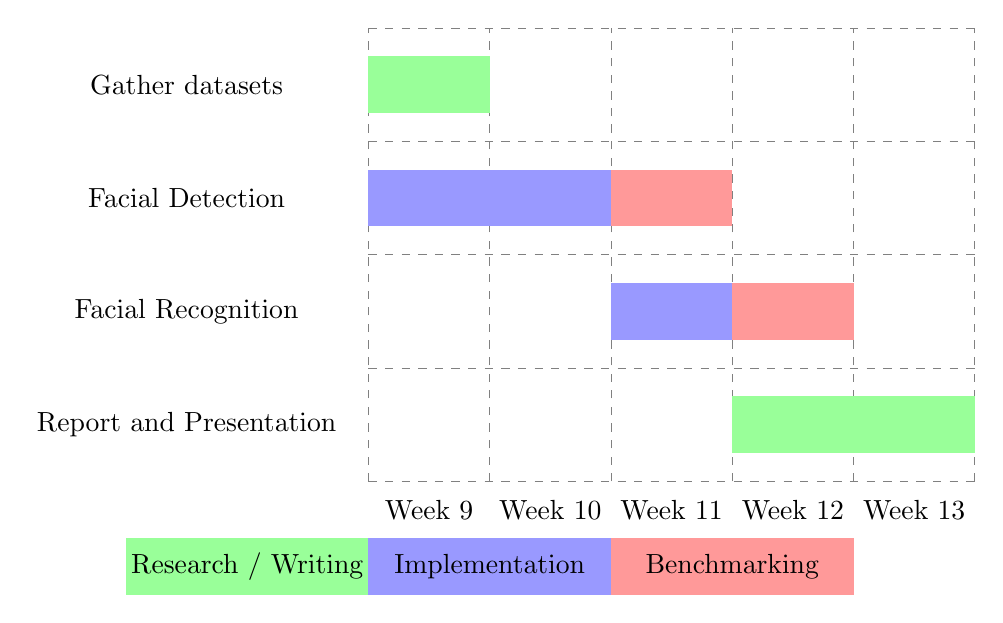
\begin{tikzpicture}[xscale=0.77,yscale=0.72]

  \draw[step=2cm,gray,very thin,dashed] (0,0) grid (10,8);
  \node[] at (1,-0.5) {Week 9};
  \node[] at (3,-0.5) {Week 10};
  \node[] at (5,-0.5) {Week 11};
  \node[] at (7,-0.5) {Week 12};
  \node[] at (9,-0.5) {Week 13};

  % datasets
  \node[] at (-3, 7) {Gather datasets};
  \fill[green!40!white] (0,6.5) rectangle (2,7.5);

  % SIFT feature detection + Eigen faces  
  \node[] at (-3, 5) {Facial Detection};
  \fill[blue!40!white] (0,4.5) rectangle (4,5.5);
  \fill[red!40!white] (4,4.5) rectangle (6,5.5);

  % ranking
  \node[] at (-3, 3) {Facial Recognition};
  \fill[blue!40!white] (4,2.5) rectangle (6,3.5);
  \fill[red!40!white] (6,2.5) rectangle (8,3.5);

  % documentation
  \node[] at (-3, 1) {Report and Presentation};
  \fill[green!40!white] (6,0.5) rectangle (10,1.5);

  % legend
  \fill[green!40!white] (-4, -2) rectangle (0, -1);
  \node[] at (-2, -1.5) {Research / Writing};
  \fill[blue!40!white] (0, -2) rectangle (4, -1);
  \node[] at (2, -1.5) {Implementation};
  \fill[red!40!white] (4, -2) rectangle (8, -1);
  \node[] at (6, -1.5) {Benchmarking};

\end{tikzpicture}
\end{figure}

\end{frame}

\begin{frame}[allowframebreaks]
	\frametitle{References}
	\bibliographystyle{plain}
	\bibliography{../bibliography}
\end{frame}

\end{document} 